\chapter{Evaluation of \glsentrytext{bosss} for Viscid Flows}
\label{viscousCylinder}
In this chapter, we aim at validating \gls{bosss} for viscid flows with \gls{ibm}s. In order to have a good comparable result, we will once again regard the flow around a cylinder as in chapter \cref{eulerVerification}. 
The viscous flow around a cylinder has been approached by many papers both experimentally and numerically, e.g. \textcite{williamson1996vortex}, \textcite{FLM:14223}, \textcite{canutoTaira}, though very few numerical approaches use a \gls{rkdg} method combined with immersed boundaries. In order to validate the \gls{bosss} code with immersed boundaries not only for the Euler equations as we did in chapter \cref{eulerVerification} but also for the viscous case we will now consider different Reynolds numbers for the steady and unsteady flow and compare our results to those of other studies.

\section{Theory}
	The flow around a viscous cylinder can be divided into different sections depending on the Reynolds number as shown in \cref{fig:overview}. The first section applies for Reynolds numbers $0 < \text{Re} < 40-50$ characterised by a laminar steady flow. In that regime, a recirculation region with two symmetric vortices with opposite directions is comprised by the wake. The flow can be described using the wake separation length $W^*$.\\\\
	\begin{figure}[htp]
		\centering
		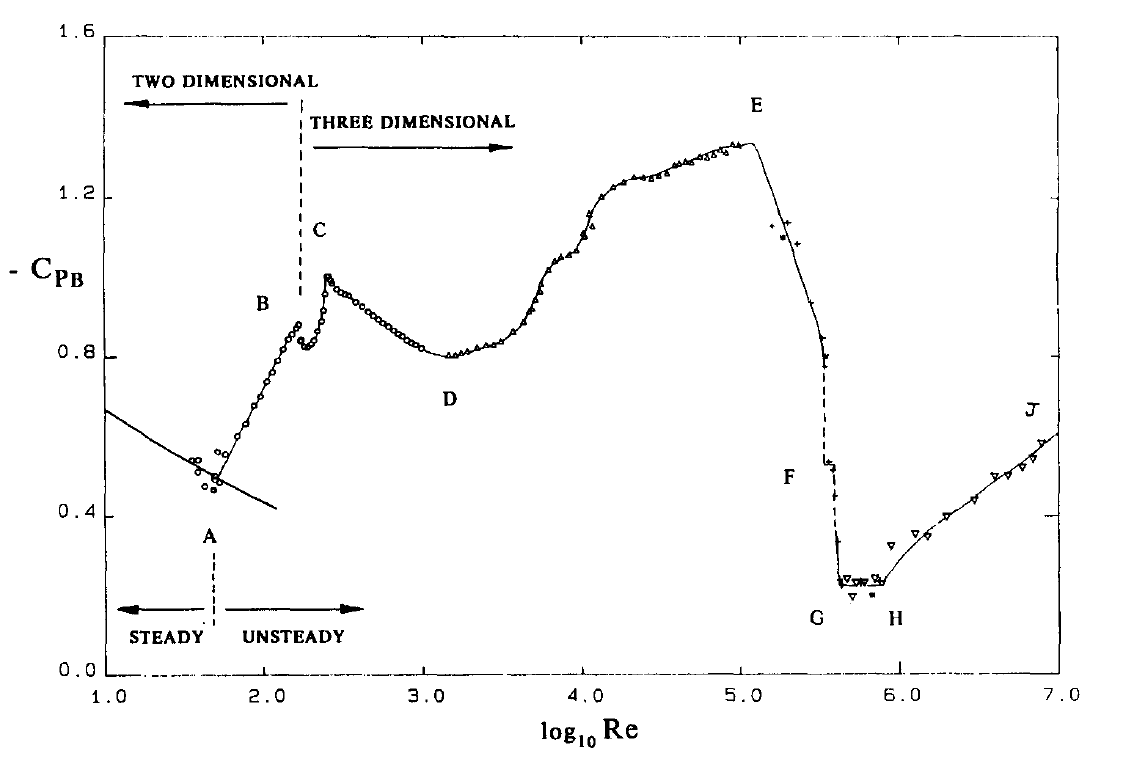
\includegraphics[height=8cm]{overviewCylinderReynolds_Williamson.PNG}
		\caption{Overview of Base Suction Coefficients over Reynolds Number \cite{williamson1996vortex}}
		\label{fig:overview}
	\end{figure} 
	The second section contains all other Reynolds number $\text{Re}> 40-50$ and thus describes the unsteady flow. It can be subdivided in several subsections \cite{williamson1996vortex}:
	\begin{itemize}
		\item $40-50 < \text{Re} < 190$: laminar vortex shedding,
		\item $190 < \text{Re} < 260$: \gls{3d} wake-transition regime,
		\item $260 < \text{Re} < 1000$: increasing disorder in the fine-scale three-dimensionalities,
		\item $1000 < \text{Re} < 200000$: shear layer transition regime,
		\item $200000 < \text{Re}$: critical transition, supercritical regime and post-critical regime.
	\end{itemize}
	
	As we will only discuss Reynolds numbers up to $\text{Re} = 200$, the important phases for us are the laminar steady regime and the laminar vortex shedding. At around $\text{Re} = 190$, the three dimensionality of the system has an incrementing influence on the flow; for we only analyse the \gls{2d} model of the experiment we stop at $\text{Re} = 200$ expecting slight deflection in our results.
	
	\subsection{The Laminar Steady Regime}
	
	At Reynolds numbers below 50, the flow forms a steady recirculation region, characterised by the wake separation length  $W^*$. It is built by two symmetrically placed vortices on each side of the wake as can be seen in \cref{fig:steady}. It has been shown experimentally as well as numerically that the wake separation length increases with increasing Reynolds number. 
		\begin{figure}[htp]
			\centering
			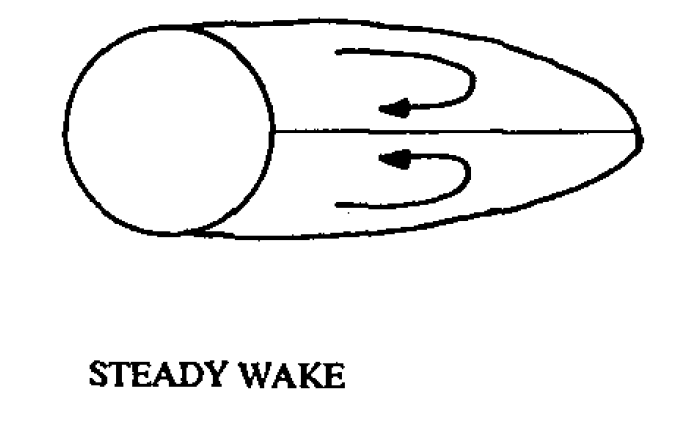
\includegraphics[height=4cm]{steadyFlow_Williamson.PNG}
			\caption{Recirculation Region \cite{williamson1996vortex}}
			\label{fig:steady}
		\end{figure}
	\subsection{Laminar Vortex Shedding}
	For Reynolds numbers of between 50 and 200 the recirculation region develops instabilities leading to the development of turbulence in the wake. This results into fully periodic vortex shedding, known as the Kármán vortex street, as can be seen in \cref{fig:unsteady}. With increasing Reynolds number the amplitudes of the drag and lift coefficients increase while the Strouhal number and frequency, respectively, decrease.
	
		\begin{figure}[htp]
			\centering
			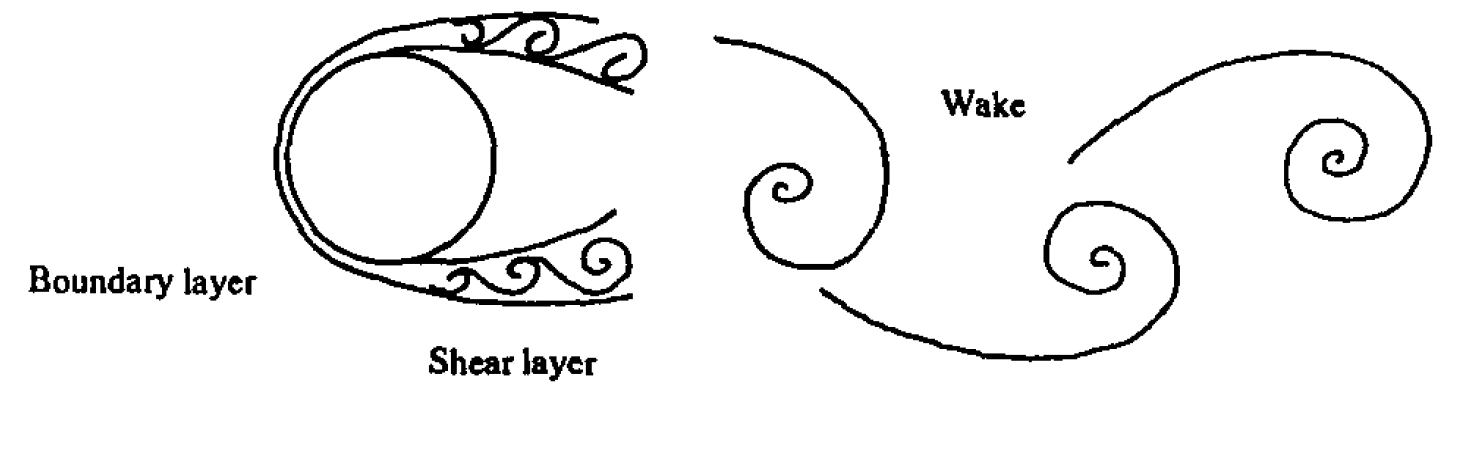
\includegraphics[height=4cm]{unsteady_Williamson.PNG}
			\caption{Kármán Vortex Street \cite{williamson1996vortex}}
			\label{fig:unsteady}
		\end{figure}
		
\section{Simulations}
	In this section we will compare the lift and drag coefficients $C_L$ and $C_D$ at different Reynolds numbers and mesh sizes at a constant agglomeration threshold of $0.3$, different polynomial degrees of 1, 2 and 3 and meshes of $40 \times 40$, $60 \times 60$ and $80 \times 80$ cells. The meshes can be found in the appendix. \\\indent
	The different simulation properties will be abbreviated as DG $+$ \textit{polynomial degree} $+$ CpD $+$ \textit{number of cells per direction}, e.g. DG2CpD80 for a simulation with polynomial degree 2 and $80 \times 80$ cells.\\
	In \cref{DOF} you can see the total \gls{dof} for each simulation taking into account the \gls{dof}s produced by order 1, 2 and 3 with 3, 6 and 10 \gls{dof}s per cell.
	
	\begin{table}[htp]
		\centering
		\def\arraystretch{1.5}
			\begin{tabular}{|c|c|c|c|c|}
				\hline
				\multicolumn{2}{|c|}{\multirow{2}{*}{DoF}} & \multicolumn{3}{c|}{CpD} \\ \cline{3-5} 
				\multicolumn{2}{|c|}{}                       & 40     & 60    & 80    \\ \hline
				\multirow{3}{*}{DG}            & 1           &    4800    &    10800   &    19200    \\ \cline{2-5} 
				& 2           &    9600    &   21600    &    38400    \\ \cline{2-5} 
				& 3           &      16000  &   36000    &   64000     \\ \hline
			\end{tabular}
			\caption{Degrees of Freedom for Different Simulation Properties}	
			\label{DOF}
	\end{table}
	During the evaluation of our results, we will also compare simulations of similar \gls{dof}s like DG2CpD40 and DG1CpD60 or DG3CpD60 and DG2CpD80 in order to inspect the influence of higher order and finer mesh properties.
	
	 The drag and lift coefficients are defined as
	\begin{align}
		C_D = \dfrac{d}{q_\infty L_\infty} \\
		C_L = \dfrac{l}{q_\infty L_\infty}
	\end{align}
	with the dynamic pressure $q_\infty = \dfrac{1}{2} \rho_\infty V_\infty^2$. For we set $L_\infty = \rho_\infty = V_\infty = 1$ in our boundary and initial conditions, we can assume
	\begin{align}
		C_D = 2 \cdot d \\
		C_L = 2 \cdot l,
	\end{align}
	with the drag and lift forces $d$ and $l$ provided from the calculation. \\\\
	As we expect asymmetrical oscillations of the flow with higher Reynolds numbers, we cannot limit the domain to the upper or lower half as we did in \cref{eulerVerification}. In order to reduce the runtime of the calculations, we will compute a smaller domain with $-20 \leq x \leq 20$, $-20 \leq y \leq 20$ and the cylinder radius $r = 0.5$ during the simulations.
	We will use a rectilinear mesh that is finer near the cylinder with the level set $\varphi = x^2 + y^2 -0.5^2$, an isothermal wall boundary condition at the cylinder wall and supersonic inlet boundary conditions for the domain borders that shall prevent the reflection of the initial wave.  \\\\
		
	\subsection{Steady State Simulations ($\text{Re} < 40-50$)}
	For the steady state simulations, we can use the wake separation length $W^*$ as an additional variable to compare to other simulations.
			\begin{figure}[htp]
				\centering
				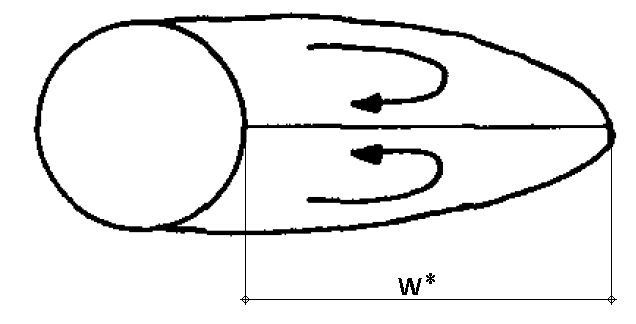
\includegraphics[height=4cm]{steadyFlow_modifiedWilliamson.PNG}
				\caption{Wake separation length, taken from \cite{williamson1996vortex}, modified }
				\label{fig:wakeSeparation}
			\end{figure} 
	It can be found from examining the x-velocity $U$ at $y=0$; the x-position where $U$ changes its sign should be the end position of the wake.

	\subsubsection{Simulation at Reynolds Number 20}
	We will now simulate the flow at $\text{Re}=20$ and compare our results to several experimental and numerical results as shown in \cref{tab:table20}. The results are divided into three categories: experimental, numerical incompressible and numerical compressible in order to coincide with the arrangement given by \textcite{ayers}.Furthermore the results are divided into \gls{2d} and \gls{3d} simulations which should not produce large differences as long as we are regarding low Reynolds numbers. The values that were produced by \textcite{brehm2015locally} using $\text{Ma} = 0.1$ as well as those that were simulated as incompressible flows can still be compared as in these low Mach numbers the compressibility does not have a great effect on the flow.

\begin{table}[htp]
	\centering
	\begin{tabular}{|l|l|c|c|c|}
		\hline
		\rule{0pt}{2,3ex}$\text{Re}=20$                              & Source                             & \gls{2d}/\gls{3d} & $W^*$ & $C_D$ \\ \hline
		\rule{0pt}{2,3ex}\multirow{3}{*}{\begin{minipage}{2.8cm}Numerical --\newline Incompressible\end{minipage}} & \textcite{dennis1970numerical}           & \gls{2d}    & $0.94$     & $2.05$     \\ \cline{2-5} 
		\rule{0pt}{2,3ex}& \textcite{fornberg1980numerical}                 & \gls{2d}    & $0.91$     & $2.00$     \\ \cline{2-5} 
		\rule{0pt}{2,3ex}&\textcite{linnick2005high}          & \gls{2d}    &$ 0.93 $    & $2.06$     \\ \hline
		\rule{0pt}{2,3ex}\multirow{2}{*}{Experimental}               & \textcite{coutanceau1977experimental}       & -     & 0.93    & -     \\ \cline{2-5} 
		\rule{0pt}{2,3ex}& \textcite{tritton1959experiments}             & -     & -     & $2.09$     \\ \hline
		\rule{0pt}{2,3ex}\multirow{3}{*}{\begin{minipage}{2.8cm}Numerical --\newline Compressible\end{minipage}}     & \textcite{brehm2015locally} (Ma = 0.1) & \gls{3d}    & $0.96$     &$ 2.02$     \\ \cline{2-5} 
		\rule{0pt}{2,3ex}& \textcite{ayers}                 & \gls{2d}    & $0.975$     & $2.06 $    \\ \cline{2-5} 
		\rule{0pt}{2,3ex}& \textbf{Present Results:}                   & \gls{2d}    & $0.928$     & $2.136$     \\ \hline
	\end{tabular}	
	\caption{Comparison of Results for $W^*$ and $C_D$, taken from \cite{ayers}, modified}
	\label{tab:table20} 
\end{table}

For the comparison of our values, we will take the results of our best simulation DG3CpD60. As we can see in \cref{tab:table20}, the values for the coefficient of drag are in pretty good agreement though they show a tendency of being too high. The simulated wake separation length is very accurate. \\\indent
In \cref{C_D20,W20} you can see all of the results that we got by our simulations.  

\begin{table}[htp]
	\centering
	\def\arraystretch{1.5}
%	\begin{minipage}[b]{0.3\textwidth}	
			\begin{tabular}{|c|c|c|c|c|}
				\hline
				\multicolumn{2}{|c|}{\multirow{2}{*}{$C_D$}} & \multicolumn{3}{c|}{CpD} \\ \cline{3-5} 
				\multicolumn{2}{|c|}{}                       & 40     & 60    & 80    \\ \hline
				\multirow{3}{*}{DG}            & 1           &    $1.812$    &  $1.952$     &    $1.988$    \\ \cline{2-5} 
				& 2           &    $2.141$    &    $2.138$   &   $2.197$     \\ \cline{2-5} 
				& 3           &    $2.136$    &     $2.136$  &   -     \\ \hline
			\end{tabular}
			\caption[$C_D$ Values for each simulation]{$C_D$ Values for Each Simulation ($\text{Re} = 20$)}	
			\label{C_D20}
		\end{table}
			\begin{table}[htp]
		\centering
		\def\arraystretch{1.5}
%	\end{minipage}
%	\centering
%	\quad
%	\begin{minipage}[b]{0.3\textwidth}	
		\begin{tabular}{|c|c|c|c|c|}
			\hline
			\multicolumn{2}{|c|}{\multirow{2}{*}{$W^*$}} & \multicolumn{3}{c|}{CpD} \\ \cline{3-5} 
			\multicolumn{2}{|c|}{}                       & 40     & 60    & 80    \\ \hline
			\multirow{3}{*}{DG}            & 1           &    $0.956$    &     $1.044$  &    $0.927$    \\ \cline{2-5} 
			& 2           &    $0.887$    &     $0.943$  &    $0.916$    \\ \cline{2-5} 
			& 3           &     $0.921$   &     $0.928$  &    -    \\ \hline
		\end{tabular}
		\caption{Wake Separation Lengths for Each Simulation ($\text{Re} = 20$)}	
		\label{W20}
%	\end{minipage}
\end{table}
We did not simulate DG3CPD80 as it would have taken much longer, being the simulation on the finest mesh with the highest order, than the other simulations. What is striking about our values is the discordant value of DG2CpD80 which should have been the most accurate simulation. 
Figure \ref{fig:C_D20} graphically presents the values of \cref{C_D20} and shows that higher degrees produce much faster accurate results than finer meshes. \\\indent
	\begin{figure}[htp]	
		\centering
		\begin{tikzpicture}
		\begin{semilogxaxis}[xlabel ={Cells per Direction}, ylabel ={$C_D$},  grid =major, legend entries ={$P=1$, $P = 2$, $P=3$}, unbounded coords=jump, legend style = {cells = {anchor=east}, legend pos=outer north east,}, scaled x ticks = false, scaled y ticks = false, xmin = 40, xmax = 80]
		\addplot table[ x = ms, y =dg1] {data/re20.dat};
		\addlegendentry{$P=1$}
		\addplot table[ x = ms, y =dg2] {data/re20.dat};
		\addlegendentry{$P=2$}
		\addplot table[ x = ms, y =dg3] {data/re20.dat};
		\addlegendentry{$P=3$}
		%		\addplot[mark=none, red] coordinates {(32, 1.6) (128, 1.6)};
		%		\addlegendentry{Constant Value}
		\end{semilogxaxis}	
		\end{tikzpicture}
		\caption{Graphical Presentation of Table \ref{C_D20} for $\text{Re} = 20$}
		\label{fig:C_D20}	
	\end{figure}
	In \cref{fig:C_Dt} you can see the behaviour of the coefficient of drag over time for different simulations. The peak at the beginning is produced because the flow reacts to the cylinder that is suddenly put into place at $t=0$. Afterwards the value drops quickly; at around $t=10$ the almost steady state is reached, though the $C_D$ value is still slightly falling. We stopped the simulation at $t=14$ so we could better compare the result to the one of \textcite{ayers}. It is to be assumed that for a longer simulation time the flow would reach the completely steady state and the coefficient of drag would finally converge to the expected value. The examination of its behaviour for a longer simulated physical time shall be subject of future works.\\\indent
\begin{figure}[htp]	
	\centering
	\begin{tikzpicture}
	\begin{semilogyaxis}[xlabel ={Time}, ylabel ={$C_D$},  grid =major, unbounded coords=jump, legend style = {cells = {anchor=east}, legend pos=outer north east}, scaled x ticks = false, scaled y ticks = false, xmin = 0, xmax = 14]
	\addplot[brown] table[x = t, y =C_D, mark=none] {data/re20dg1cpd40.dat};
	\addlegendentry{DG1CpD40}
	\addplot[red] table[ x = t, y =C_D, mark=none] {data/re20dg2cpd60.dat};
	\addlegendentry{DG2CpD60}
	\addplot[blue] table[ x = t, y =C_D, mark=none] {data/re20dg3cpd60.dat};
	\addlegendentry{DG3CpD60}
	\addplot[black] table[ x = t, y =C_D, mark=none] {data/re20dg2cpd80.dat};
	\addlegendentry{DG2CpD80}
	%		\addplot[mark=none, red] coordinates {(32, 1.6) (128, 1.6)};
	%		\addlegendentry{Constant Value}
	\end{semilogyaxis}	
	\end{tikzpicture}
	\caption{Coefficient of Drag over Time ($\text{Re} = 20$)}
	\label{fig:C_Dt}	
\end{figure}
We will conclude the examination of the flow for $\text{Re} = 20$ with the visualisation of the vorticity for DG3CpD60  in \cref{fig:vorticity20}.
	
\begin{figure}[htp]
	\centering
	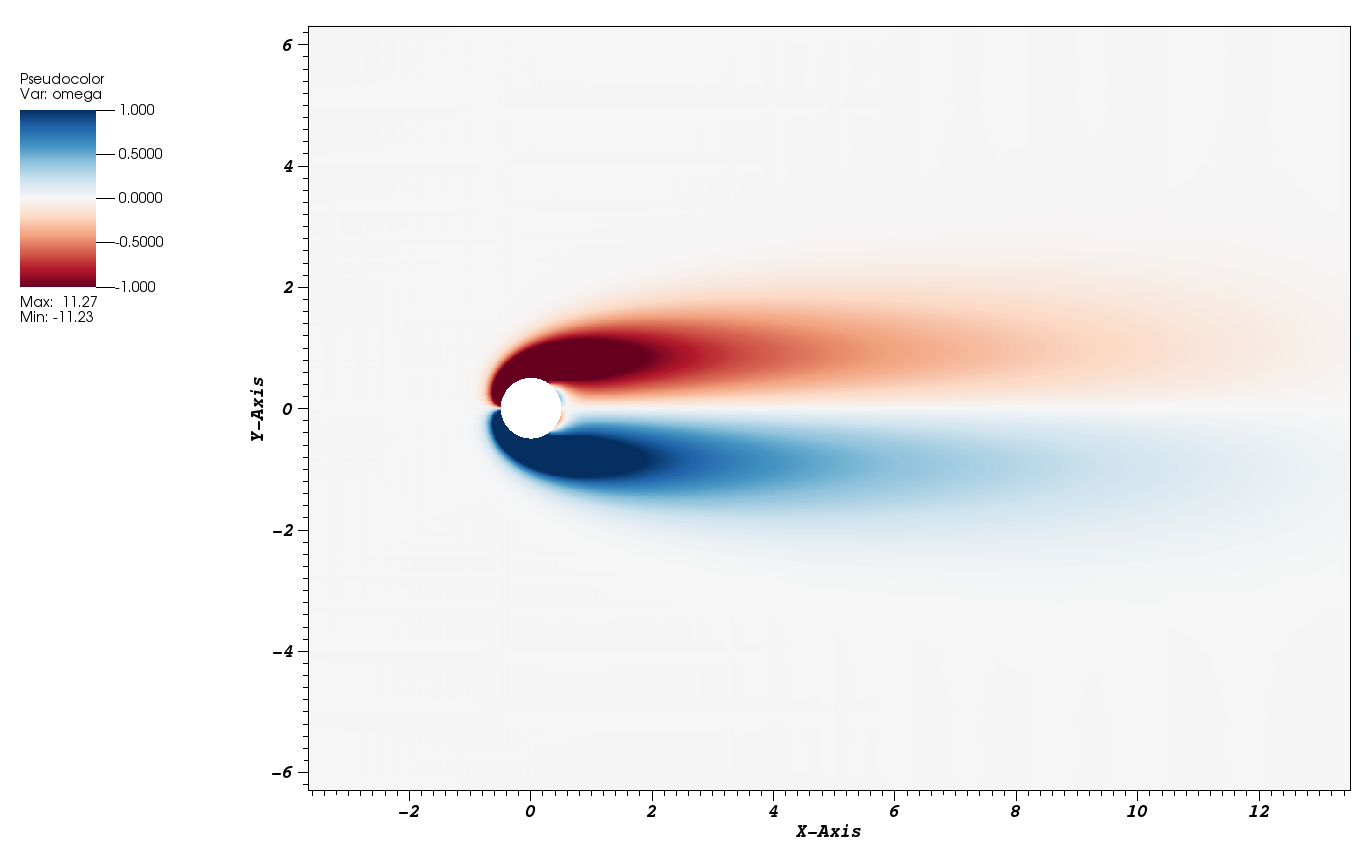
\includegraphics[height=10cm]{Re20DG3CpD60.png}
	\caption{Vorticity for DG3CpD60 for $\text{Re} = 20$}
	\label{fig:vorticity20}
\end{figure}	

	\subsubsection{Simulation at Reynolds Number 40}
	As we did for $\text{Re}=20$, we will now compare our results for the wake separation length and the coefficient of drag to those documented before by others. Once again, we compare our result simulated with DG3CpD60 which now is much more accurate than it was for $\text{Re}=20$. Both the coefficient of drag and the wake separation length are in very good agreement with the other values; the coefficient of drag is slightly higher while the wake separation length is slightly lower than the results we are comparing to. As we expected before, we can confirm the theory that higher Reynolds number cause higher wake separation lengths.
\begin{table}[htp]
	\centering
	\begin{tabular}{|l|l|c|c|c|}
		\hline
		\rule{0pt}{2,3ex}$\text{Re}=40$                              & Source                             & \gls{2d}/\gls{3d} & $W^*$ & $C_D$ \\ \hline
		\rule{0pt}{2,3ex}\multirow{3}{*}{\begin{minipage}{2.8cm}Numerical --\newline Incompressible\end{minipage}} &\textcite{dennis1970numerical}           & \gls{2d}    & $2.35$     & $1.52 $    \\ \cline{2-5} 
		\rule{0pt}{2,3ex}& \textcite{fornberg1980numerical}                & \gls{2d}    & $2.24$     & $1.50 $   \\ \cline{2-5} 
		\rule{0pt}{2,3ex}& \textcite{linnick2005high}          & \gls{2d}    &$ 2.28$     & $1.54  $   \\ \hline
		\rule{0pt}{2,3ex}\multirow{2}{*}{Experimental}               & \textcite{coutanceau1977experimental}      & -     & $2.13 $  & -     \\ \cline{2-5} 
		\rule{0pt}{2,3ex}& \textcite{tritton1959experiments}                 & -     & -     & $1.59 $    \\ \hline
		\rule{0pt}{2,3ex}\multirow{3}{*}{\begin{minipage}{2.8cm}Numerical --\newline Compressible\end{minipage}}     & \textcite{brehm2015locally} (Ma = 0.1) & \gls{3d}    & $2.26$     & $1.51 $    \\ \cline{2-5} 
		\rule{0pt}{2,3ex}& \textcite{ayers}                  & \gls{2d}    & $2.250 $    & $1.605$     \\ \cline{2-5} 
		\rule{0pt}{2,3ex}& \textbf{Present Results:}                   & \gls{2d}    & $2.201$     & $1.608 $    \\ \hline
	\end{tabular}	
	\caption{Comparison of Results for $W^*$ and $C_D$, taken from \cite{ayers}, modified}
	\label{table40}
\end{table}
In \cref{C_D40,W40}, you can see the results of every simulation. As we did for $\text{Re}=20$, we did not simulate DG3CpD80 as it would have taken too long. Unfortunately, we did not get a stable calculation for DG3CpD40 until we reduced the time step by ninety-five per cent. This resulted into a tremendous runtime which made the simulation impossible. \\\indent
\begin{table}[htp]
	\centering
	\def\arraystretch{1.5}
%	\begin{minipage}[b]{0.3\textwidth}	
		\begin{tabular}{|c|c|c|c|c|}
			\hline
			\multicolumn{2}{|c|}{\multirow{2}{*}{$C_D$}} & \multicolumn{3}{c|}{CpD} \\ \cline{3-5} 
			\multicolumn{2}{|c|}{}                       & 40     & 60    & 80    \\ \hline
			\multirow{3}{*}{DG}            & 1           &   $1.373$     &     $1.461$  &     $1.485$   \\ \cline{2-5} 
			& 2           &     $1.600$   &   $1.596$    &     $1.616$   \\ \cline{2-5} 
			& 3           &      -  &     $1.608$  &     -   \\ \hline
		\end{tabular}
		\caption[$C_D$ Values for each simulation]{$C_D$ Values for Each Simulation ($\text{Re} = 40$)}	
		\label{C_D40}
	\end{table}
	\begin{table}[htp]
	\centering
	\def\arraystretch{1.5}
%	\end{minipage}
%	\centering
%	\quad
%	\begin{minipage}[b]{0.3\textwidth}	
		\begin{tabular}{|c|c|c|c|c|}
			\hline
			\multicolumn{2}{|c|}{\multirow{2}{*}{$W^*$}} & \multicolumn{3}{c|}{CpD} \\ \cline{3-5} 
			\multicolumn{2}{|c|}{}                       & 40     & 60    & 80    \\ \hline
			\multirow{3}{*}{DG}            & 1           &    $2.342$    &    $2.338$   &    $2.236$    \\ \cline{2-5} 
			& 2           &     $2.115$   &    $2.182$   &     $2.182$   \\ \cline{2-5} 
			& 3           &     -   &    $2.201$   &    -    \\ \hline
		\end{tabular}
		\caption{Wake Separation Lengths for Each Simulation ($\text{Re} = 40$)}	
		\label{W40}
%	\end{minipage} 
\end{table}
In \cref{fig:C_D40} you can see the graphical presentation of \cref{C_D40}; here it is very clear that higher order calculations provide even for coarse meshes very accurate solutions. \\\indent
	\begin{figure}[htp]	
		\centering
		\begin{tikzpicture}
		\begin{semilogxaxis}[xlabel ={Cells per Direction}, ylabel ={$C_D$},  grid =major, legend entries ={$P=1$, $P = 2$, $P=3$}, unbounded coords=jump, legend style = {cells = {anchor=east}, legend pos=outer north east,}, scaled x ticks = false, scaled y ticks = false, xmin = 40, xmax = 80]
		\addplot table[ x = ms, y =dg1] {data/re40.dat};
		\addlegendentry{$P=1$}
		\addplot table[ x = ms, y =dg2] {data/re40.dat};
		\addlegendentry{$P=2$}
		\addplot table[ x = ms, y =dg3] {data/re40.dat};
		\addlegendentry{$P=3$}
%		\addplot[mark=none, red] coordinates {(32, 1.6) (128, 1.6)};
%		\addlegendentry{Constant Value}
		\end{semilogxaxis}	
		\end{tikzpicture}
		\caption{Graphical Presentation of Table \ref{C_D40} for $\text{Re} = 40$}
		\label{fig:C_D40}	
	\end{figure}
\begin{figure}[htp]	
	\centering
	\begin{tikzpicture}
	\begin{semilogyaxis}[xlabel ={Time}, ylabel ={$C_D$},  grid =major, unbounded coords=jump, legend style = {cells = {anchor=east}, legend pos=outer north east}, scaled x ticks = false, scaled y ticks = false, xmin = 0, xmax = 14]
	\addplot[brown] table[x = t, y =C_D, mark=none] {data/re40dg1cpd40.dat};
	\addlegendentry{DG1CpD40}
	\addplot[red] table[ x = t, y =C_D, mark=none] {data/re40dg2cpd60.dat};
	\addlegendentry{DG2CpD60}
	\addplot[blue] table[ x = t, y =C_D, mark=none] {data/re40dg3cpd60.dat};
	\addlegendentry{DG3CpD60}
	\addplot[black] table[ x = t, y =C_D, mark=none] {data/re40dg2cpd80.dat};
	\addlegendentry{DG2CpD80}
	%		\addplot[mark=none, red] coordinates {(32, 1.6) (128, 1.6)};
	%		\addlegendentry{Constant Value}
	\end{semilogyaxis}	
	\end{tikzpicture}
	\caption{Coefficient of Drag over Time ($\text{Re} = 40$)}
	\label{fig:C_Dt40}	
\end{figure}
As you can see in \cref{fig:C_Dt40}, the behaviour of the coefficient of drag over the physical time is very similar for the simulations plotted. They are more in agreement with each other than they were for $\text{Re = 20}$. In \cref{fig:vorticity40}, you can see the vorticity for DG3CpD60; there we remark that the wake is much longer than it was for $\text{Re}=20$.
\begin{figure}[htp]
	\centering
	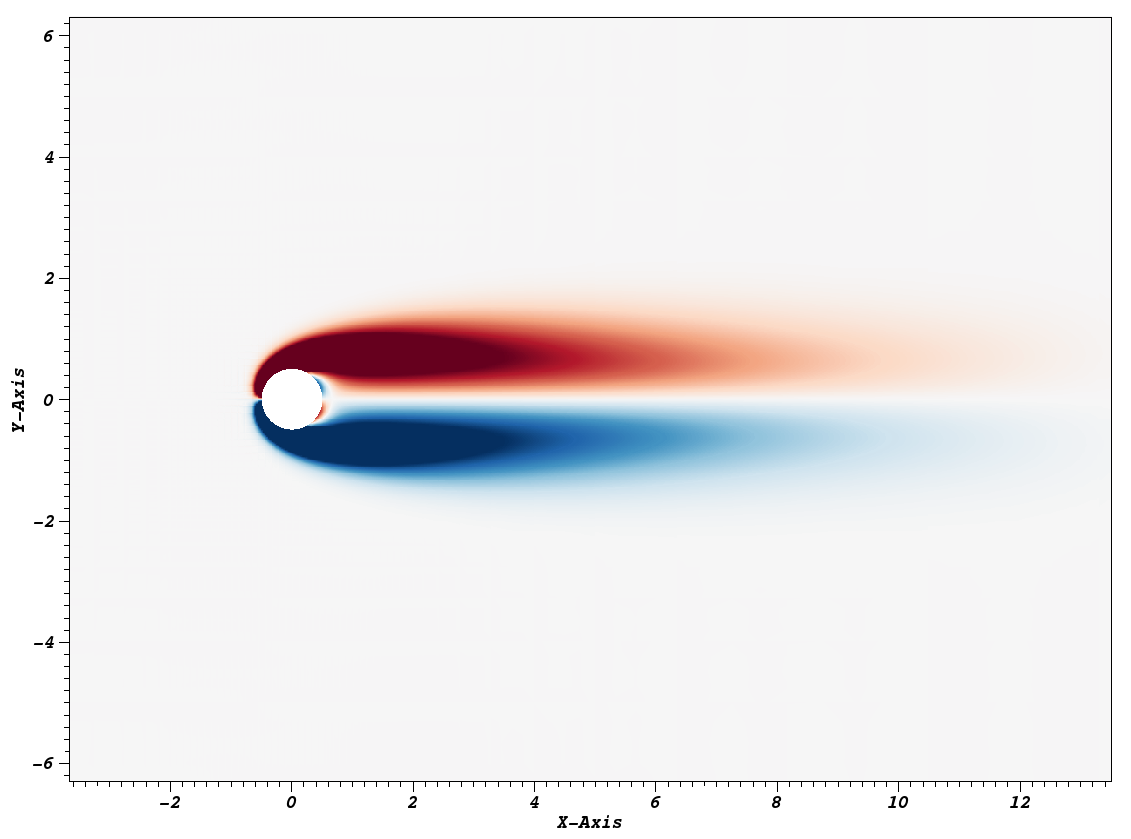
\includegraphics[height=10cm]{Re40DG3CpD60.png}
	\caption{Vorticity for DG3CpD60 for $\text{Re} = 40$}
	\label{fig:vorticity40}
\end{figure}
	\subsection{Unsteady Simulations ($\text{Re}> 40-50$)}
	After having examined the steady simulations which were very accurate for the coefficient of drag, we will now turn to the unsteady ones with $\text{Re}=100$ and $\text{Re}=200$.
	In order to compare the unsteady simulations, we need the Strouhal number
	\begin{align}
		\text{St} = \dfrac{f  L_\infty}{V_\infty}.
	\end{align}
	As our initial and boundary conditions give $V_\infty = L_\infty = 1$, we can calculate $\text{St} = f$ with $f$ found from examining the oscillation of $C_L$ over time. In order to develop vortex shedding, the flow needs small perturbations that destabilise the flow towards a symmetry breaking state (\textcite{FLM:14223}). In reality those are given by the structure of the cylinder, the influence of the walls or the not completely straight inflow; in our simulations they come from small truncation errors and the computer's round-off errors. 
	In order to accelerate the process until the wake begins to oscillate, one could also start the flow with a vortex that induces a high perturbation much earlier. For it did not take long until the wake began to oscillate it was not needed in our simulations.
	\subsubsection{Simulation at Reynolds Number 100}
	In the following, we will compare the coefficients of lift and drag as well as the Strouhal number. As you can see in \cref{table100}, the produced results are once again very accurate and in good agreement with those of other studies. All of our results for the best calculation DG3CpD60 lie perfectly in the range that has been given by other studies.  The overview of all collected values can be found in \cref{CL100,C_D100,Str100}. They are written as mean value plus/minus amplitude in order to show the oscillation of lift and drag. We can clearly observe that DG1CpD40 produces very inaccurate results; as soon as either mesh fineness or \gls{dg} order is increased, we immediately receive very good results. Furthermore we observe that the higher-order results of those with the same \gls{dof}s yield better results than those with a finer mesh.
\begin{table}[H]
	\centering
	\begin{tabular}{|l|p{4cm}|c|c|c|c|}
		\hline
		\rule{0pt}{2,3ex}$\text{Re}=100$                              & Source                             & \gls{2d}/\gls{3d} & $St$ & $C_D$ & $C_L$\\ \hline
		\rule{0pt}{2,3ex}\multirow{7}{*}{\begin{minipage}{2.8cm}Numerical --\newline Incompressible\end{minipage}} & \textcite{gresho1984modified}           & \gls{2d}    & $0.18$     & $1.76$ & -   \\ \cline{2-6} 
		\rule{0pt}{2,3ex}&\textcite{linnick2005high} \newline ($\lambda = 0.056$)                 & \gls{2d}    & $0.169$     & $1.38 \pm 0.010$  &  $\pm  0.337 $\\ \cline{2-6} 
		\rule{0pt}{2,3ex}&\textcite{linnick2005high} \newline ($\lambda = 0.023$)                  & \gls{2d}    & $0.1696 $   & $1.34 \pm 0.009$  & $ \pm 0.333 $\\ \cline{2-6} 
		\rule{0pt}{2,3ex}&\textcite{FLM:14223}                  & \gls{2d}    & $0.165  $   &$ 1.253 $ & -  \\ \cline{2-6} 
		\rule{0pt}{2,3ex}& \textcite{saiki1996numerical}                 & \gls{2d}    &$ 0.171  $   & $1.26 $ &  - \\ \cline{2-6} 
		\rule{0pt}{2,3ex}& \textcite{FLM:14223}                    & \gls{3d}    & $0.164$     & $1.240 $ & -  \\ \cline{2-6} 
		\rule{0pt}{2,3ex}& \textcite{liu1998preconditioned}          & \gls{3d}    &$ 0.165 $    & $1.35 \pm 0.012$  &$ \pm 0.339 $ \\ \hline
		\rule{0pt}{2,3ex}\multirow{2}{*}{Experimental}               & \textcite{berger1972periodic}     & -     &$ 0.16-0.17 $   & -    & -\\ \cline{2-6} 
		\rule{0pt}{2,3ex}& \textcite{clift2005bubbles}                & -    & -     &$ 1.24 $ &  - \\ \cline{2-6} 
		\rule{0pt}{2,3ex}& \textcite{williamson1996vortex}               & -     &$ 0.164  $  & -   & - \\ \hline
		\rule{0pt}{2,3ex}\multirow{3}{*}{\begin{minipage}{2.8cm}Numerical -- \newline Compressible\end{minipage}}     & \textcite{brehm2015locally} \newline (Ma = 0.1) & \gls{3d}    & $0.165$    &$ 1.32 \pm 0.01  $  & $\pm 0.32 $\\ \cline{2-6} 
		\rule{0pt}{2,3ex}& \textcite{ayers}                  & \gls{2d}    &$ 0.167$     & $1.371 \pm 0.011 $ &$ \pm 0.333 $\\ \cline{2-6} 
		\rule{0pt}{2,3ex}& \textbf{Present Results:}                   & \gls{2d}    & $0.1669$     & $1.3593 \pm 0.00805$  &  $\pm 0.3291$ \\ \hline
	\end{tabular}	
	\caption{Comparison of Results for $St$, $C_D$ and $C_L$, taken from \cite{ayers}, modified}
	\label{table100}
\end{table}



\begin{table}[H]
	\centering
	\def\arraystretch{1.5}
	%	\begin{minipage}[b]{0.3\textwidth}	
	\begin{tabular}{|c|c|c|c|c|}
		\hline
		\multicolumn{2}{|c|}{\multirow{2}{*}{$C_D$}} & \multicolumn{3}{c|}{CpD} \\ \cline{3-5} 
		\multicolumn{2}{|c|}{}                       & 40     & 60    & 80    \\ \hline
		\multirow{3}{*}{DG}            & 1           &   $0.9777\pm 0.0003$     &     $1.2 \pm 0.0834$  &     $1.233 \pm 0.0118$   \\ \cline{2-5} 
		& 2           &     $1.291 \pm 0.0082$   &   $1.3156 \pm 0.0089$    &     $1.3501 \pm 0.0079$   \\ \cline{2-5} 
		& 3           &      -  &     $1.3593 \pm 0.00805$   &     -   \\ \hline
	\end{tabular}
	\caption[$C_D$ Values for Each simulation]{$C_D$ Values for Each Simulation ($\text{Re} = 100$)}	
	\label{C_D100}
\end{table}
\begin{table}[H]
	\centering
	\def\arraystretch{1.5}
	%	\end{minipage}
	%	\centering
	%	\quad
	%	\begin{minipage}[b]{0.3\textwidth}	
	\begin{tabular}{|c|c|c|c|c|}
		\hline
		\multicolumn{2}{|c|}{\multirow{2}{*}{$C_L$}} & \multicolumn{3}{c|}{CpD} \\ \cline{3-5} 
		\multicolumn{2}{|c|}{}                       & 40     & 60    & 80    \\ \hline
		\multirow{3}{*}{DG}            & 1           &    $\pm 0.00155$    &    $\pm 0.291$   &    $\pm 0.2789$    \\ \cline{2-5} 
		& 2           &     $\pm 0.2672$   &    $\pm 0.3154$   &     $\pm 0.3135$   \\ \cline{2-5} 
		& 3           &     -   &    $\pm 0.3291$  &    -    \\ \hline
	\end{tabular}
	\caption{$C_L$ Values for Each Simulation ($\text{Re} = 100$)}	
	\label{CL100}
	%	\end{minipage} 
\end{table}
\begin{table}[H]
	\centering
	\def\arraystretch{1.5}
	%	\end{minipage}
	%	\centering
	%	\quad
	%	\begin{minipage}[b]{0.3\textwidth}	
	\begin{tabular}{|c|c|c|c|c|}
		\hline
		\multicolumn{2}{|c|}{\multirow{2}{*}{St}} & \multicolumn{3}{c|}{CpD} \\ \cline{3-5} 
		\multicolumn{2}{|c|}{}                       & 40     & 60    & 80    \\ \hline
		\multirow{3}{*}{DG}            & 1           &    $0.1001$    &    $0.1506$   &    $0.1502$    \\ \cline{2-5} 
		& 2           &     $0.1669$   &    $0.1669$   &     $0.1670$   \\ \cline{2-5} 
		& 3           &     -   &    $0.1669$   &    -    \\ \hline
	\end{tabular}
	\caption{Strouhal Numbers for Each Simulation ($\text{Re} = 100$)}	
	\label{Str100}
	%	\end{minipage} 
\end{table}
\newpage
%\cref{fig:C_D100} graphically presents \cref{C_D100} and shows that higher order calculations immediately yield good results. This time, there is no such discordant value for DG2CpD80 which is higher than it should be as appeared for $\text{Re}=20$ and $\text{Re}=40$. 
%	\begin{figure}[htp]	
%		\centering
%		\begin{tikzpicture}
%		\begin{semilogxaxis}[xlabel ={Cells per Direction}, ylabel ={$C_D$},  grid =major, legend entries ={$P=1$, $P = 2$, $P=3$}, unbounded coords=jump, legend style = {cells = {anchor=east}, legend pos=outer north east,}, scaled x ticks = false, scaled y ticks = false, xmin = 40, xmax = 80]
%		\addplot table[ x = ms, y =dg1] {data/re100.dat};
%		\addlegendentry{$P=1$}
%		\addplot table[ x = ms, y =dg2] {data/re100.dat};
%		\addlegendentry{$P=2$}
%		\addplot table[ x = ms, y =dg3] {data/re100.dat};
%		\addlegendentry{$P=3$}
%		%		\addplot[mark=none, red] coordinates {(32, 1.6) (128, 1.6)};
%		%		\addlegendentry{Constant Value}
%		\end{semilogxaxis}	
%		\end{tikzpicture}
%		\caption{Graphical Presentation of Table \ref{C_D100} for $\text{Re} = 100$}
%		\label{fig:C_D100}	
%	\end{figure}

In \cref{osci100} the coefficient of lift over time is presented. It shows that at around $t=90s$ amplitude and frequency stay the same, though regarding 
\cref{cdosci100} the coefficient of drag reaches the constant oscillation state at around $t=110s$. These plots were produced with the results from DG3CpD60. They also show that the frequency of $C_D$ is twice as high as the frequency of the lift coefficient. 
\begin{figure}[htp]	
	\centering
	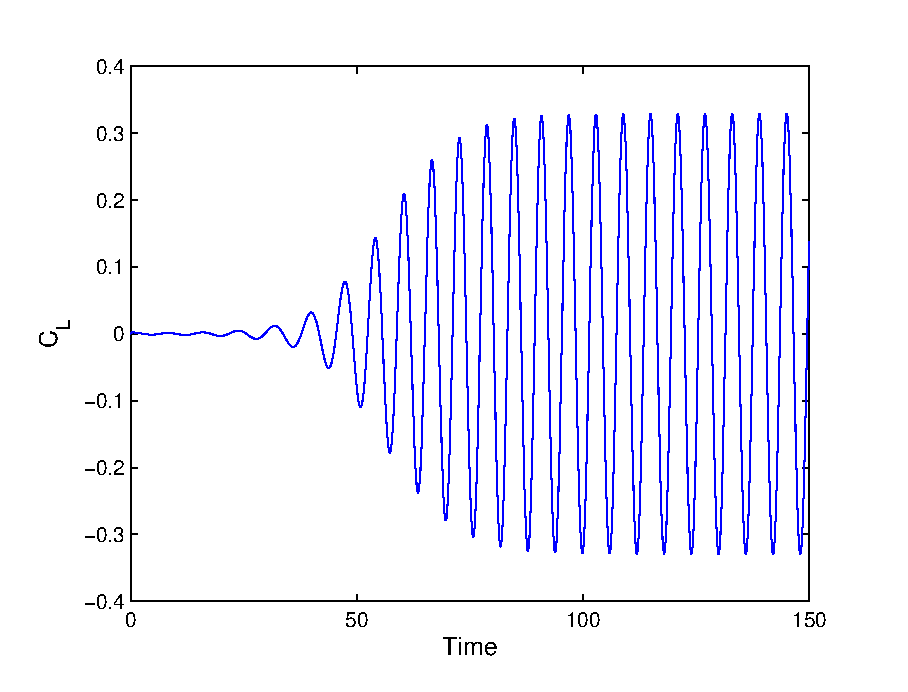
\includegraphics[height=8cm]{re100dg3cpd60cl.eps}
	\caption{Lift coefficient over time for $0s<t<150s$ ($\text{Re}=100$)}
	\label{osci100}	
\end{figure}
\begin{figure}[htp]	
	\begin{minipage}[b]{0.45\textwidth}
		\centering
		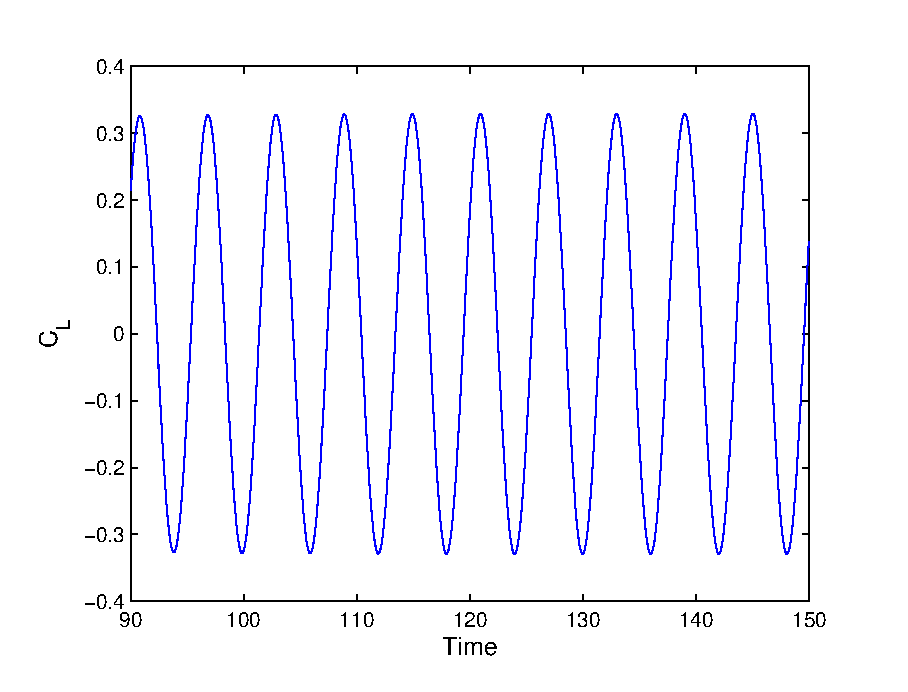
\includegraphics[height=6cm]{re100dg3cpd60cl90.eps}
		\caption{Lift coefficient over time for $90s<t<150s$ ($\text{Re}=100$)}
		\label{cl10090}
	\end{minipage}
	\quad
	\begin{minipage}[b]{0.45\textwidth}
		\centering
		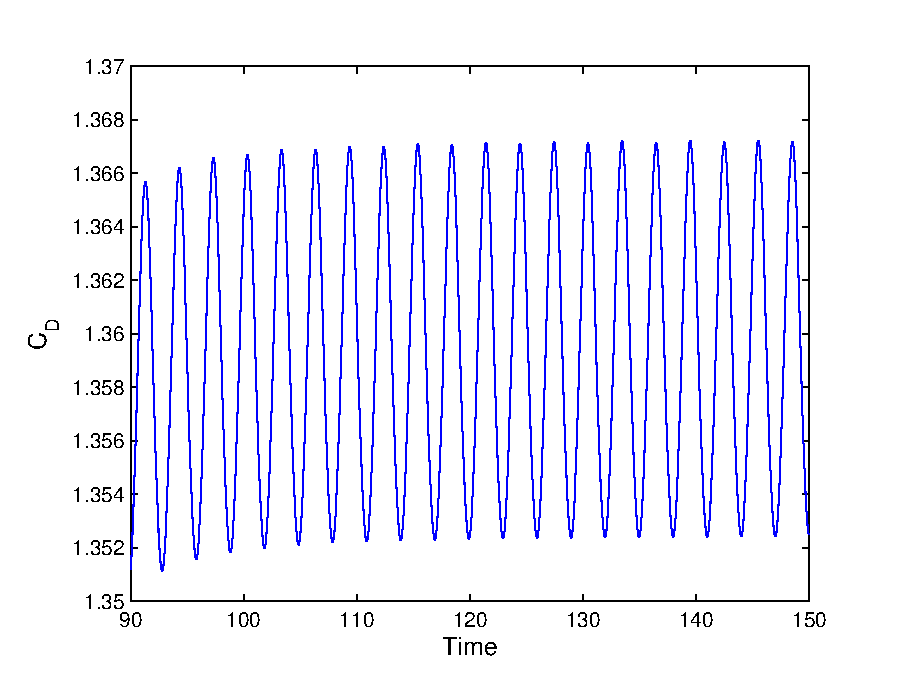
\includegraphics[height=6cm]{re100dg3cpd60cd90.eps}
		\caption{Drag coefficient over time for $90s<t<150s$ ($\text{Re}=100$)}
		\label{cdosci100}	
	\end{minipage}
\end{figure}
	
%		\begin{figure}[htp]	
%			\centering
%			\begin{tikzpicture}
%				\begin{axis}[xlabel ={Time}, ylabel ={$C_L$}]%, grid =major, legend entries ={$P=1$}, unbounded coords=jump, legend style = {cells = {anchor=east}, legend pos=outer north east,}, scaled x ticks = false, xmin = 0, xmax = 120]
%				\addplot table[ x = time, y = l, mark=none] {data/re100dg2cpd60cl.dat};
%				\end{axis}	
%			\end{tikzpicture}
%			\caption{Lift coefficient over time for $0s<t<150s$ ($\text{Re}=100$)}
%			\label{osci100}	
%		\end{figure}
%\begin{figure}[htp]	
%	\begin{minipage}[b]{0.45\textwidth}
%			\centering
%			\begin{tikzpicture}
%			\begin{axis}[xlabel ={Time}, ylabel ={$C_L$},  grid =major, unbounded coords=jump, legend style = {cells = {anchor=east}, legend pos=outer north east,}, scaled x ticks = false, scaled y ticks = false, xmin = 90, xmax = 150]
%			\addplot table[ x =time, y =l, mark=none] {data/re100dg2cpd60cl.dat};
%			\end{axis}	
%			\end{tikzpicture}
%			\caption{Lift coefficient over time for $90s<t<150s$ ($\text{Re}=100$)}
%			\label{shijfterror}	
%	\end{minipage}
%	\begin{minipage}[b]{0.45\textwidth}
%			\centering
%			\begin{tikzpicture}
%			\begin{axis}[xlabel ={Time}, ylabel ={$C_D$},  grid =major,  legend style = {cells = {anchor=east}, legend pos=outer north east,}, restrict x to domain=90:150, xmin = 90, xmax = 150]
%			\addplot table[ x =time, y =d, mark=none] {data/re100dg2cpd60cd.dat};
%			\end{axis}	
%			\end{tikzpicture}
%			\caption{Drag coefficient over time for $90s<t<150s$ ($\text{Re}=100$)}
%			\label{cdosci100}	
%	\end{minipage}
%\end{figure}
		
		We will conclude the evaluation of the simulation at Reynolds number 100 with a visualisation of the vorticity for DG2CpD60 in \cref{fig:vorticity100}. As we used a very coarse mesh outside $-2\leq x,y \leq 2$ the vortices get stretched in the wake and there are sharp jumps at the cell edges. By observing the vorticity over time, we could conclude that the Strouhal number, which describes the frequency of the vortex shedding, can be found from examining the coefficient of lift as vortex shedding and lift changes appeared in the exact same frequency.
		\begin{figure}[htp]
			\centering
			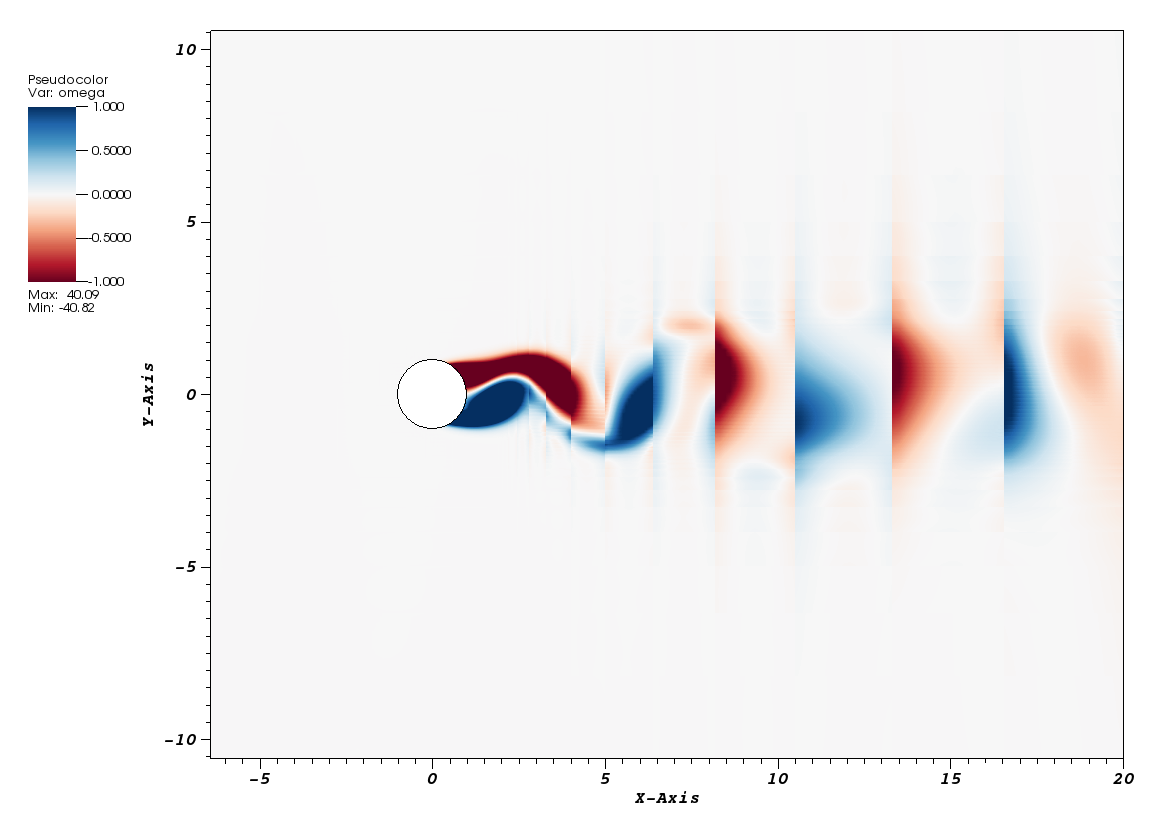
\includegraphics[height=10cm]{re100dg3cpd60.png}
			\caption{Vorticity for DG3CpD60 for $\text{Re} = 100$}
			\label{fig:vorticity100}
		\end{figure}
		
		\newpage
	\subsubsection{Simulation at Reynolds Number 200}
	Finally, we will come to the simulation at $\text{Re}=200$. Once again, the results that we received are accurate and in good agreement, as can be seen in \cref{table200}. Compared to $\text{Re}=100$ the frequency of the vortex shedding as well as the amplitude of the coefficient of lift increased while the coefficient of drag stayed at about the same.  Compared to the three dimensional simulations by \textcite{brehm2015locally}, our results for the coefficient of drag are slightly higher, as we only did \gls{2d} simulations.  All of our results can be found in \cref{C_D200,CL200,Str200}.
\begin{table}[htp]
	\centering
	\begin{tabular}{|l|p{3.5cm}|c|c|c|c|}
		\hline
		\rule{0pt}{2,3ex}$\text{Re}=200$                              & Source                             & \gls{2d}/\gls{3d} & $St$ & $C_D$ & $C_L$\\ \hline
		\rule{0pt}{2,3ex}\multirow{9}{*}{\begin{minipage}{2.8cm}Numerical --\newline Incompressible\end{minipage}} & \textcite{belov1995new}            & \gls{2d}    & $0.193$     & $1.19 \pm 0.042$ & $\pm 0.64$   \\ \cline{2-6} 
		\rule{0pt}{2,3ex} & \textcite{gresho1984modified}             & \gls{2d}    & $0.21$     & $1.76$ & -   \\ \cline{2-6} 
		\rule{0pt}{2,3ex}&\textcite{linnick2005high} \newline ($\lambda = 0.056$)                 & \gls{2d}    & $0.199$     & $1.37 \pm 0.046$  &  $\pm  0.70$\\ \cline{2-6} 
		\rule{0pt}{2,3ex}&\textcite{linnick2005high} \newline ($\lambda = 0.023$)                  & \gls{2d}    & $0.197 $   & $1.34 \pm 0.044$  & $ \pm 0.69$\\ \cline{2-6} 
		\rule{0pt}{2,3ex}& \textcite{miyake1992numerical}               & \gls{2d}    & $0.196$   &$1.34 \pm 0.043 $ & $\pm 0.67$  \\ \cline{2-6} 
		\rule{0pt}{2,3ex}&  \textcite{FLM:14223}               & \gls{2d}    & $0.198  $   &$ 1.321 $ & -  \\ \cline{2-6} 
		\rule{0pt}{2,3ex}&\textcite{saiki1996numerical}                 & \gls{2d}    &$ 0.197  $   & $1.18 $ &  - \\ \cline{2-6} 
		\rule{0pt}{2,3ex}& \textcite{FLM:14223}                   & \gls{3d}    & $0.181$     & $1.306 $ & -  \\ \cline{2-6} 
		\rule{0pt}{2,3ex}&\textcite{liu1998preconditioned}           & \gls{3d}    &$ 0.192 $    & $1.31 \pm 0.049$  &$ \pm 0.69 $ \\ \hline
		\rule{0pt}{2,3ex}\multirow{2}{*}{Experimental}               & \textcite{berger1972periodic}      & -     &$ 0.18-0.19 $   & -    & -\\ \cline{2-6} 
		\rule{0pt}{2,3ex}& \textcite{clift2005bubbles}                  & -    & -     &$ 1.16 $ &  - \\ \cline{2-6} 
		\rule{0pt}{2,3ex}& \textcite{williamson1996vortex}               & -     &$ 0.181  $  & -   & - \\ \hline
		\rule{0pt}{2,3ex}\multirow{3}{*}{\begin{minipage}{2.8cm}Numerical --\newline Compressible\end{minipage} }    &  \textcite{brehm2015locally} \newline (Ma = 0.1) & \gls{3d}    & $0.192$    &$ 1.3 \pm 0.04  $  & $\pm 0.66 $\\ \cline{2-6} 
		\rule{0pt}{2,3ex}& \textcite{ayers}                   & \gls{2d}    &$ 0.201$     & $1.371 \pm 0.011 $ &$ \pm 0.70 $\\ \cline{2-6} 
		\rule{0pt}{2,3ex}& \textbf{Present Results:}                   & \gls{2d}    & $0.2002$     & $1.344 \pm 0.0462$  &   $\pm 0.6887$\\ \hline
	\end{tabular}	
	\caption{Comparison of Results for $St$, $C_D$ and $C_L$, taken from \cite{ayers}, modified}
	\label{table200}
\end{table}

\begin{table}[htp]
	\centering
	\def\arraystretch{1.5}
	%	\begin{minipage}[b]{0.3\textwidth}	
	\begin{tabular}{|c|c|c|c|c|}
		\hline
		\multicolumn{2}{|c|}{\multirow{2}{*}{$C_D$}} & \multicolumn{3}{c|}{CpD} \\ \cline{3-5} 
		\multicolumn{2}{|c|}{}                       & 40     & 60    & 80    \\ \hline
		\multirow{3}{*}{DG}            & 1           &   $0.8144\pm 0.0028$     &     $1.2427 \pm 0.0281$  &     $1.2256 \pm 0.0309$   \\ \cline{2-5} 
		& 2           &     $1.2508 \pm 0.0339$   &   $1.3593 \pm 0.0080$    &     $1.3501 \pm 0.0079$   \\ \cline{2-5} 
		& 3           &      -  &     $1.344 \pm 0.0462$   &     -   \\ \hline
	\end{tabular}
	\caption[$C_D$ Values for Each simulation]{$C_D$ Values for Each Simulation ($\text{Re} = 200$)}	
	\label{C_D200}
\end{table}
\begin{table}[htp]
	\centering
	\def\arraystretch{1.5}
	%	\end{minipage}
	%	\centering
	%	\quad
	%	\begin{minipage}[b]{0.3\textwidth}	
	\begin{tabular}{|c|c|c|c|c|}
		\hline
		\multicolumn{2}{|c|}{\multirow{2}{*}{$C_L$}} & \multicolumn{3}{c|}{CpD} \\ \cline{3-5} 
		\multicolumn{2}{|c|}{}                       & 40     & 60    & 80    \\ \hline
		\multirow{3}{*}{DG}            & 1           &    $\pm 3.2629 \cdot 10^{-5}$    &    $\pm 0.5304$   &    $\pm 0.2789$    \\ \cline{2-5} 
		& 2           &     $\pm 0.5653$   &    $\pm 0.6433$   &     $\pm 0.6376$   \\ \cline{2-5} 
		& 3           &     -   &    $\pm 0.6887$  &    -    \\ \hline
	\end{tabular}
	\caption{$C_L$ Values for Each Simulation ($\text{Re} = 200$)}	
	\label{CL200}
	%	\end{minipage} 
\end{table}
\begin{table}[htp]
	\centering
	\def\arraystretch{1.5}
	%	\end{minipage}
	%	\centering
	%	\quad
	%	\begin{minipage}[b]{0.3\textwidth}	
	\begin{tabular}{|c|c|c|c|c|}
		\hline
		\multicolumn{2}{|c|}{\multirow{2}{*}{St}} & \multicolumn{3}{c|}{CpD} \\ \cline{3-5} 
		\multicolumn{2}{|c|}{}                       & 40     & 60    & 80    \\ \hline
		\multirow{3}{*}{DG}            & 1           &    $0$    &    $0.1836$   &    $0.1838$    \\ \cline{2-5} 
		& 2           &     $0.2003$   &    $0.2002$   &     $0.2002$   \\ \cline{2-5} 
		& 3           &     -   &    $0.2002$   &    -    \\ \hline
	\end{tabular}
	\caption{Strouhal Numbers for Each Simulation ($\text{Re} = 200$)}	
	\label{Str200}
	%	\end{minipage} 
\end{table}
\newpage
In \cref{osci200}, we can see that the steady state is reached earlier compared to $\text{Re}=100$; the coefficient of lift settles into a state of constant amplitude and frequency at around $t=65s$. Figures \ref{cl90} and \ref{cdosci200} show the frequency and amplitude of $C_L$ and $C_D$, respectively, for the steady state from $90s \leq t \leq 150s$. There we can see that frequency and amplitude are higher compared to $\text{Re}=100$.
%\begin{figure}[htp]	
%	\centering
%	\begin{tikzpicture}
%	\begin{semilogxaxis}[xlabel ={Cells per Direction}, ylabel ={$C_D$},  grid =major, legend entries ={$P=1$, $P = 2$, $P=3$}, unbounded coords=jump, legend style = {cells = {anchor=east}, legend pos=outer north east,}, scaled x ticks = false, scaled y ticks = false, xmin = 40, xmax = 80]
%	\addplot table[ x = ms, y =dg1] {data/re200.dat};
%	\addlegendentry{$P=1$}
%	\addplot table[ x = ms, y =dg2] {data/re200.dat};
%	\addlegendentry{$P=2$}
%	\addplot table[ x = ms, y =dg3] {data/re200.dat};
%	\addlegendentry{$P=3$}
%	%		\addplot[mark=none, red] coordinates {(32, 1.6) (128, 1.6)};
%	%		\addlegendentry{Constant Value}
%	\end{semilogxaxis}	
%	\end{tikzpicture}
%	\caption{Graphical Presentation of Table \ref{C_D200} for $\text{Re} = 200$}
%	\label{fig:C_D200}	
%\end{figure}


\begin{figure}[htp]	
	\centering
	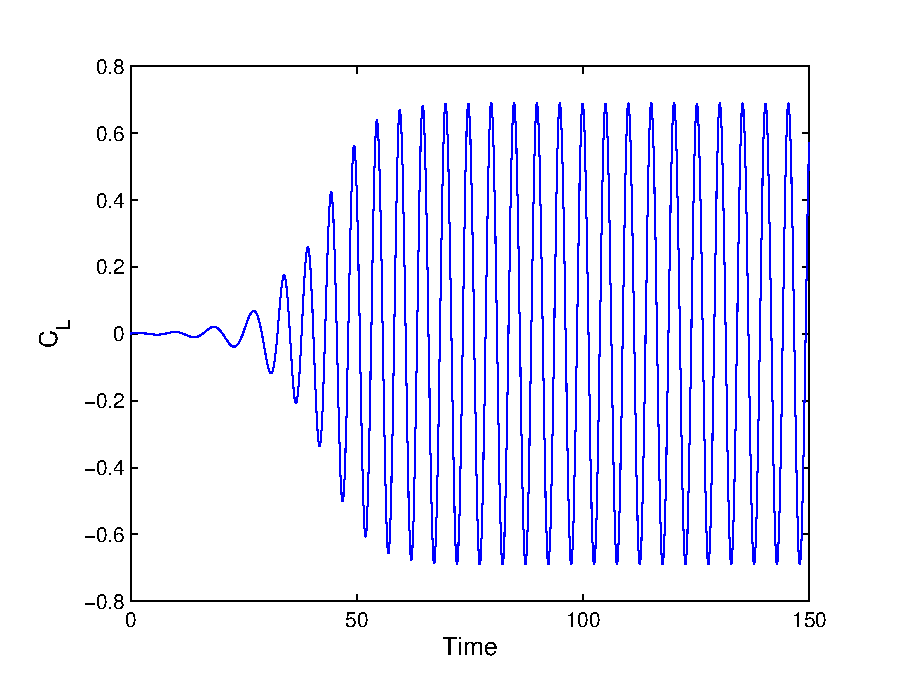
\includegraphics[height=8cm]{re200dg3cpd60cl.eps}
	\caption{Lift coefficient over time for $0s<t<150s$ ($\text{Re}=200$)}
	\label{osci200}	
\end{figure}
\begin{figure}[htp]	
	\begin{minipage}[b]{0.45\textwidth}
		\centering
		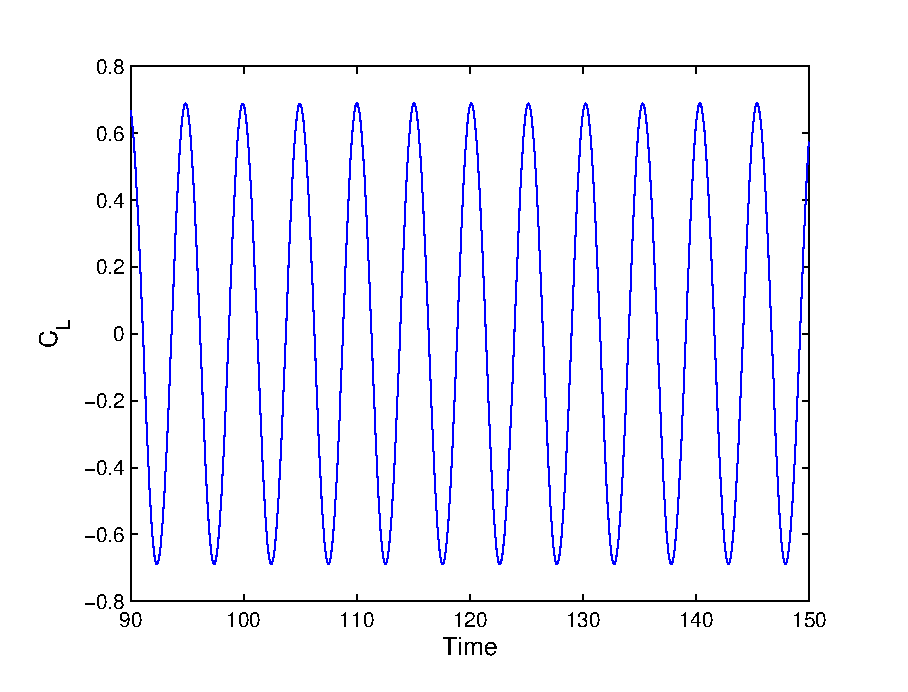
\includegraphics[height=6cm]{re200dg3cpd60cl90.eps}
		\caption{Lift coefficient over time for $90s<t<150s$ ($\text{Re}=200$)}
		\label{cl90}
	\end{minipage}
	\quad
	\begin{minipage}[b]{0.45\textwidth}
		\centering
		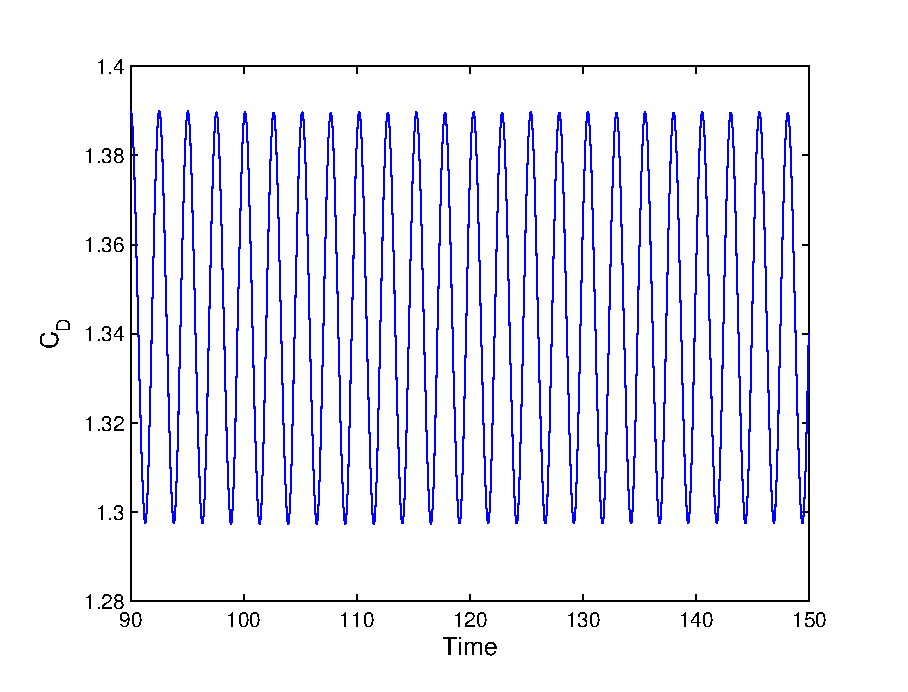
\includegraphics[height=6cm]{re200dg3cpd60cd90.eps}
		\caption{Drag coefficient over time for $90s<t<150s$ ($\text{Re}=200$)}
		\label{cdosci200}	
	\end{minipage}
\end{figure}
\newpage
We will conclude the simulation part of this work with the visualisation of the vorticity for $\text{Re}=200$ in \cref{fig:vorticity200}. We can observe that the amount of vortices has increased. Unfortunately the mesh is too coarse to properly show the wake of the cylinder.
\begin{figure}[htp]
	\centering
	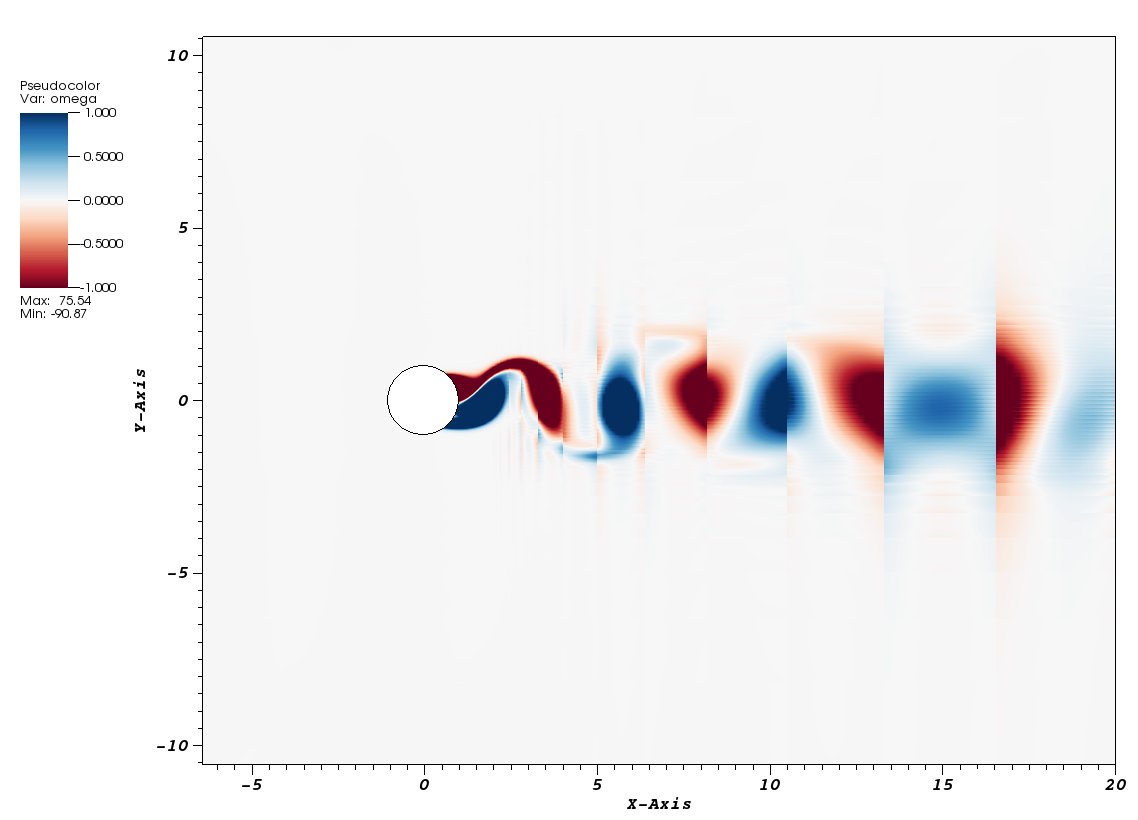
\includegraphics[height=10cm]{re200dg3cpd60.png}
	\caption{Vorticity for DG3CpD60 for $\text{Re} = 200$}
	\label{fig:vorticity200}
\end{figure}

